%%
%% Copyright 2016 Dmitry Meshkov
%%

\documentclass[number,preprint,review]{elsarticle}

%% Use the options 1p,twocolumn; 3p; 3p,twocolumn; 5p; or 5p,twocolumn
%% for a journal layout:
%% \documentclass[final,1p,times]{elsarticle}
%% \documentclass[final,1p,times,twocolumn]{elsarticle}
%% \documentclass[final,3p,times]{elsarticle}
%% \documentclass[final,3p,times,twocolumn]{elsarticle}
%% \documentclass[final,5p,times]{elsarticle}
%% \documentclass[final,5p,times,twocolumn]{elsarticle}

%% For including figures, graphicx.sty has been loaded in
%% elsarticle.cls. If you prefer to use the old commands
%% please give \usepackage{epsfig}

%% The amssymb package provides various useful mathematical symbols
\usepackage{amssymb}
%% The amsthm package provides extended theorem environments
\usepackage{amsthm}

%% for url reference
\usepackage{hyperref}
\usepackage{graphicx}

%% The lineno packages adds line numbers. Start line numbering with
%% \begin{linenumbers}, end it with \end{linenumbers}. Or switch it on
%% for the whole article with \linenumbers.
%% \usepackage{lineno}

\journal{??????????????????}

\begin{document}

\begin{frontmatter}

%% Title, authors and addresses

%% use the tnoteref command within \title for footnotes;
%% use the tnotetext command for theassociated footnote;
%% use the fnref command within \author or \address for footnotes;
%% use the fntext command for theassociated footnote;
%% use the corref command within \author for corresponding author footnotes;
%% use the cortext command for theassociated footnote;
%% use the ead command for the email address,
%% and the form \ead[url] for the home page:
%% \title{Title\tnoteref{label1}}
%% \tnotetext[label1]{}
%% \author{Name\corref{cor1}\fnref{label2}}
%% \ead{email address}
%% \ead[url]{home page}
%% \fntext[label2]{}
%% \cortext[cor1]{}
%% \address{Address\fnref{label3}}
%% \fntext[label3]{}

\title{Difficulty Control for Blockchain Systems}


%% use optional labels to link authors explicitly to addresses:
%% \author[label1,label2]{}
%% \address[label1]{}
%% \address[label2]{}

\author[iohk]{Dmitry Meshkov}
\ead{dmitry.meshkov@iohk.io}

\author[iohk]{Alexander Chepurnoy}


\address[iohk]{IOHK Research}

\begin{abstract}
\textbf{TODO}
\end{abstract}

\begin{keyword}
Blockchain \sep Decentralized consensus \sep Peer-to-peer networks \sep Proof-of-Work
\end{keyword}

\end{frontmatter}


\section{Introduction}
\label{sec:intro}

Blockchain systems have attracted a growing amount of interest from various communities after publication of Bitcoin whitepaper \cite{Nakamoto2008} in 2008.
Bitcoin security relies on the distributed protocol that maintains the blockchain, called mining, in which network nodes tries to solve computational puzzle.
Other blockchain systems may relies on different computational puzzles \cite{??} or even on virtual mining \cite{??}, while all of them use some algorithm that changes puzzle difficulty dynamically.
This algorithm for retargeting the difficulty is required to make blockchain system predictable and fix latency between blocks.

Fixed latency between blocks is important for several reasons.
Too often blocks leads to situation, when for a lot of miners block propagation time become bigger, then latency between blocks.
This leads to significant increasing of number of blockchain forks that complicates the consensus\cite{decker2013information} and reduce effective hash rate in blockchain system.
On the other hand, increasing of the latency between blocks leads to decreasing of the network throughput\cite{miller2016} and may be critical for high-loaded blockchain systems like bitcoin, where blocks are already 70\% full today\cite{armstrong2016}.
Increasing latency by 50\% in bitcoin network will mean, that some transactions will be never included into blockchain.
Moreover this will lead to infinite growth of unconfirmed transactions pool, meaning it is likely that most bitcoin transactions will not even relay, much less confirm.

Most of blockchain systems relies on quite a naive difficulty retargeting algorithm, that assumes, that total computational power, involved in mining process, don't change over time.
Using more complicated retargeting algorithms with incorrect assumptions\cite{andruiman2014} may lead to incorrect time interval between blocks even for simple case of constant hash rate as, for example, observed in Nxt, where observed mean time between blocks is ~2 times bigger, then expected in whitepaper\cite{nxt}. Moreover, too ofter difficulty recalculation leads to wide distribution of time intervals between blocks and makes blockchain system unpredictable\cite{andruiman2014}.
Varying network computational power makes this algorithms inefficient for difficulty recalculation, e.g. continuous growth of computational power leads to decreasing mean latency between blocks and average block time in Bitcoin network is ~1.07 times lower, then expected.
Noteworthy, that exponential growth of computational power, which is the situation observed in practice in accordance with Moore’s law\cite{moore2006cramming}, is the absolutely worst case (regarding the maximal block rate) possible for Bitcoin’s difficulty retargeting algorithm\cite{kraft2015difficulty}.
On the other side, target recalculation algorithm should be easy enough and use integer arithmetic for all computational steps, since all nodes in the peer-to-peer network have to agree absolutely on the calculated difficulty.

Original Bitcoin white-paper, states that the security of the system is guaranteed as long as there is no attacker in possession of half or more of the total computational power used to maintain the system \cite{Nakamoto2008}.
Most of the models used in the literature to discuss double-spending attacks assume that mining difficulty is constant \cite{??}.
However difficulty is not constant, and can be manipulated by the attacker.
The Difficulty Raising Attack, introduced in \cite{bahack2013theoretical}, enables the attacker to discard n-depth block, for any n and any attacker hash power, with probability 1 if he\footnote{For simplicity we choose to adapt the male form. This was chosen by flipping a coin.} is willing to wait enough time.
The fact that there is no way to determine whether a block have been computed on its declared time or not, have been used as part of other attacks \cite{timejacking2011, artforz2011}.
In secton \ref{sec:bit} we introduce new way of attack for blochcking systems, that manipulates difficulty for decreasing effective hash rate, required for block generation.

New researches of difficulty control proposes better functions for difficulty recalculation.
For example paper \cite{kraft2015difficulty} introduces target recalculation function, designed to work “perfectly” not just for constant hash rate but also if the hash rate grows exponentially (with a constant but unknown rate).
Since it's good for situation, observed in practice in Bitcoin network, there are still a lot of open questions for future research.
Is it possible to create such a function, suitable for random fluctuations in the hash rate?
Is it possible to create such a function, simple enough to use integer arithmetic for all computational steps?
Is it possible to create such a function, stable for attackers manipulations?

\textbf{TODO transition to newxt section}

\section{Bitcoin Mining}
\label{sec:bit}

First, let us briefly describe how the mining process works.
The original concept is described in section 4 of the Bitcoin whitepaper \cite{Nakamoto2008}, and disscussed in plenty of papers \cite{kraft2015difficulty, miller2014permacoin, eyal2014majority}.
We refer to the basic unit of mining work in Bitcoin as a scratch-off puzzle (SOP).
Miner generates candidates to the SOP by iterating thought \(nonse\) and calculating SHA-256 hash of a blocks header.
For a block to be valid it must value hash value less than the current \(target\) that is which is usually expressed in terms of the network difficulty \(D\) as \(1\over D\).
Thus, each hash attempt yields a valid block with probability \(1\over D\) and block frequency is \(R\over D\) where \(R\) is effective network hash rate.

Every \(M\) blocks (\(M=2016\) for Bitcoin) difficulty is recalculated as
\begin{equation}
D_{i+1}=D_i*{MT\over S_m}
\end{equation}
where \(T\) is expected time interval between blocks and \(S_m\) is actual time, it took to generate \(M\) blocks.
Real time (\(~ 9 min 20 sec\)) interval is less, then desired time interval \(T=10 min\) because of continiuos growth of network computational power.
Difficulty recalculation interval \(M=2016\) has been chosen in such a way to recalculate difficulty every 2 weeks, while for real network it is a bit smaller.
This time intrerval is big enough to see increasing computational power of the network: right after target recalculation block time is close to desired 10 minutes, whereas at the end of \(epoch\) it's less then 9 minutes (see figure~\ref{fig:image}).
\begin{figure}[h]
\center{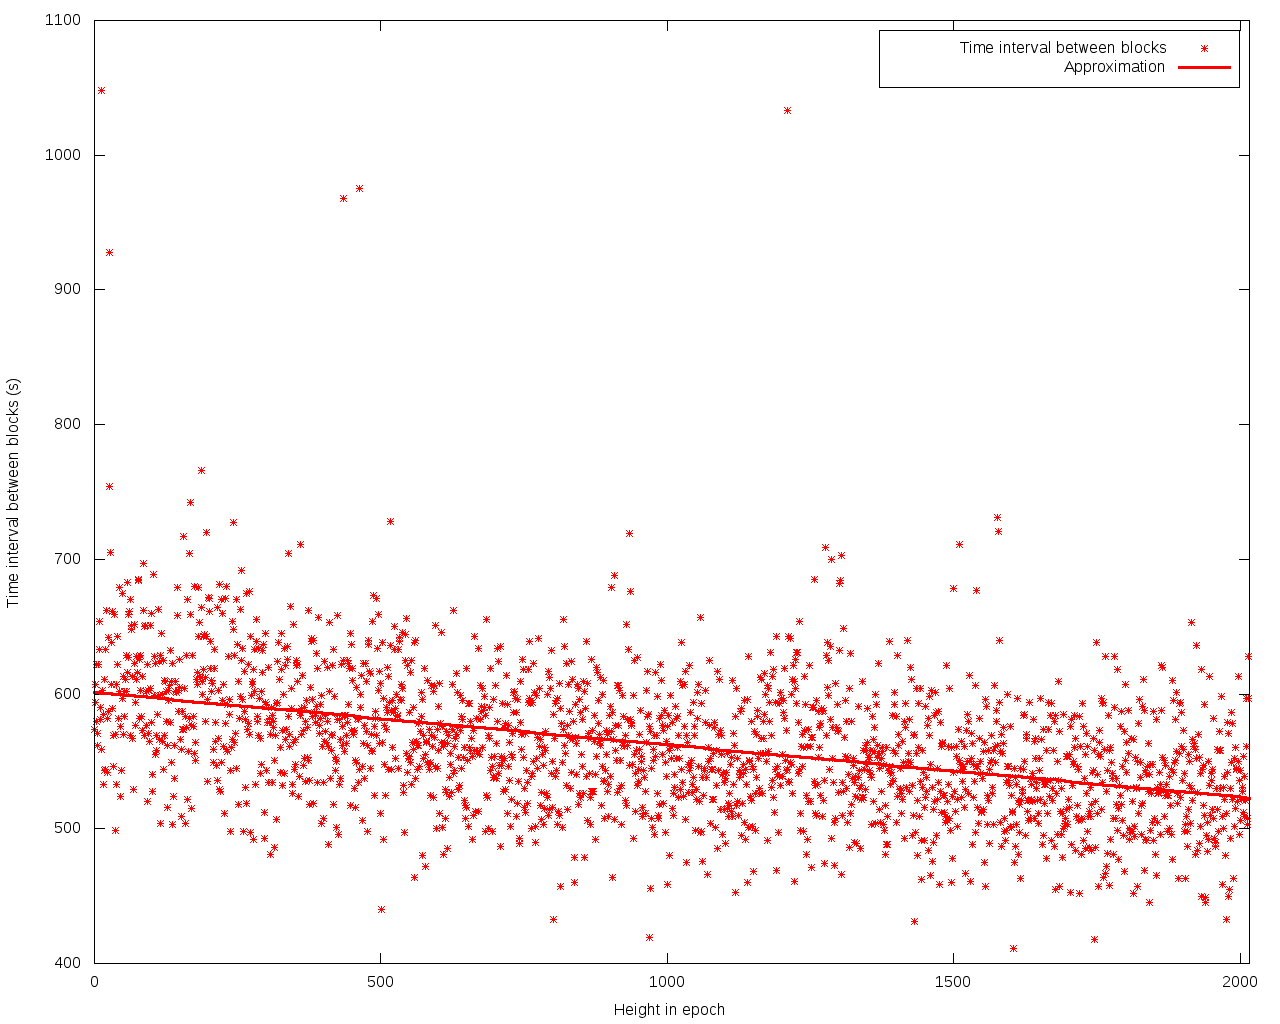
\includegraphics[scale=0.3]{interval.png}}
\caption{Average block time between difficulty recalculation}
\label{fig:image}
\end{figure}

\textbf{TODO transition to newxt section}

\section{The Difficulty Manipulating Attack}
\label{sec:attack}

On this section we show a new way of manipulating difficulty with profit to an attacker.
The main idea is very simple.
The attacker may disable his mining, and wait for the next difficulty racalculation.
New difficulty will be lower, cause it don't include computational power of the attacker, and he turns on his mining again.
After next difficulty recalculation (which will include the attacker computational power) he turns off his mining again, and wait for next difficulty recalculation.
Such a simple algorithm allows him to mine during epochs with low difficulty, and don't mine during epoch with the low one, that will decrease computational resourses expended for block generation.
Of course in such a situation the attacker will create less blocks, that in situation, when he mine all the time.
However, lows of economy dictate that the cost of computational resourses invested into mining should be around the expected reward, and attackers profit, gained from every block may overbalance his wastes caused by decreasing number of created blocks.
Moreover, in a situation with a lot cryptocurency forks he is able to mine other forks in epoches with big difficulty and gain more blocks with more profit from each, that in situation, when he mine single cryptocurrency permanently.

 \textbf{TODO subsection?}

Let's calculate attacker profit in circumstances of Bitcoin difficulty recalculation function and constant hash rate (which is natural for this function).

\section{An Improved Difficulty Control}
\label{sec:improved}

\section{Simulations}
\label{sec:sim}

\section{Conclusions}
\label{sec:concl}

\section*{References}

\bibliographystyle{elsarticle-num}
\bibliography{sources.bib}


\end{document}